\documentclass[12pt]{standalone}
\usepackage[utf8]{inputenc}
\usepackage[T1]{fontenc}
\usepackage{times}
\usepackage{amsmath,amssymb}
\usepackage[dvipsnames,svgnames]{xcolor}
\usepackage{tikz}
\usetikzlibrary{calc, positioning, arrows.meta, decorations.pathreplacing}
\definecolor{dmrsfill}{HTML}{CDE2FB}
\definecolor{winblue}{HTML}{0D366B}
\definecolor{inksec}{HTML}{52514E}
\definecolor{interf}{HTML}{C0504D}
% (a) Inicialização BDAC-MMSE (Zhao et al. 2025, Eq. 7 e paper.md:140): cada DU calcula
%     X_c = H_c^H R_cc^-1 H_c (K x K); as somas seguem a cadeia até a última DU, que inverte
%     (sum X_c + I/E_s) e envia o resultado P a todas as DUs (broadcast). Cada DU calcula
%     W_c^0 = P H_c^H R_cc^-1. Última DU que soma e inverte: modelo B (software/Restrições -
%     Parâmetros.csv, linhas 56-65).
% (b) Cadeia de DUs em cada iteração do BCD-MMSE: a DU c usa só as amostras do seu cluster e passa
%     A_c e {b_{c,i}}_{i=1}^N à seguinte; a DU C passa à DU 1 na iteração seguinte
%     (Zhao et al. 2025, Algoritmo 3 e nota 6).
\begin{document}
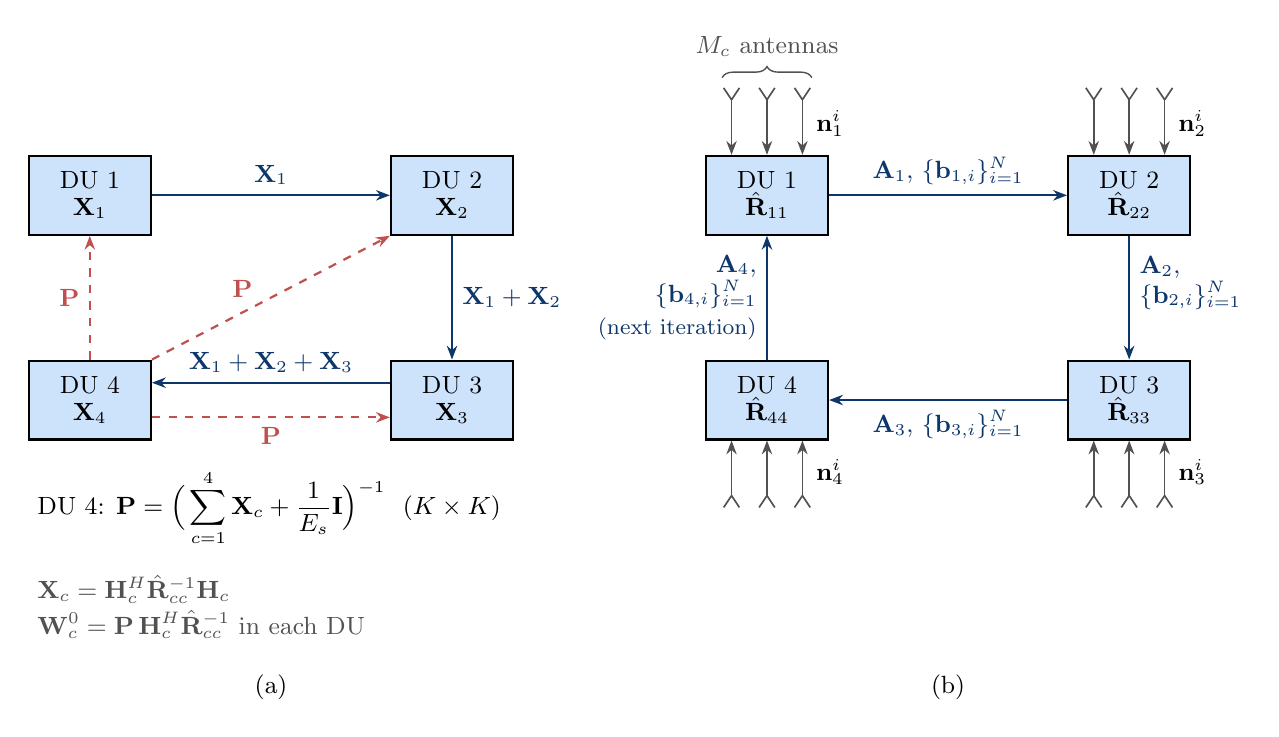
\begin{tikzpicture}[font=\fontsize{9}{10.8}\selectfont, >={Stealth[length=5pt]}]
\tikzset{du/.style={draw, line width=0.8pt, fill=dmrsfill, minimum width=1.55cm, minimum height=1.0cm, align=center}}
% ------------------------------------------------------------------ (a)
\begin{scope}[shift={(0,0)}]
  \node[du] (d1) at (0,0) {DU 1\\[-1pt]$\mathbf X_1$};
  \node[du] (d2) at (4.6,0) {DU 2\\[-1pt]$\mathbf X_2$};
  \node[du] (d3) at (4.6,-2.6) {DU 3\\[-1pt]$\mathbf X_3$};
  \node[du] (d4) at (0,-2.6) {DU 4\\[-1pt]$\mathbf X_4$};
  % somas ao longo da cadeia
  \draw[->, winblue, line width=0.8pt] (d1) -- node[above] {$\mathbf X_1$} (d2);
  \draw[->, winblue, line width=0.8pt] (d2) -- node[right] {$\mathbf X_1 + \mathbf X_2$} (d3);
  \draw[->, winblue, line width=0.8pt] ($(d3.west)+(0,0.22)$) -- node[above] {$\mathbf X_1 + \mathbf X_2 + \mathbf X_3$} ($(d4.east)+(0,0.22)$);
  % broadcast do resultado da inversão K x K
  \draw[->, interf, dashed, line width=0.8pt] ($(d4.east)+(0,-0.22)$) -- node[below] {$\mathbf P$} ($(d3.west)+(0,-0.22)$);
  \draw[->, interf, dashed, line width=0.8pt] (d4.north east) -- node[pos=0.45, above left=-2pt] {$\mathbf P$} (d2.south west);
  \draw[->, interf, dashed, line width=0.8pt] (d4) -- node[left] {$\mathbf P$} (d1);
  % o que a DU 4 calcula
  \node[below=0.25cm of d4.south west, anchor=north west, align=left] (inv)
    {DU 4: $\mathbf P = \Big(\displaystyle\sum_{c=1}^{4}\mathbf X_c + \frac{1}{E_s}\mathbf I\Big)^{-1}$ \ ($K \times K$)};
  \node[below=0.12cm of inv.south west, anchor=north west, align=left, inksec]
    {$\mathbf X_c = \mathbf H_c^H\hat{\mathbf R}_{cc}^{-1}\mathbf H_c$\\[2pt]
     $\mathbf W_c^0 = \mathbf P\,\mathbf H_c^H\hat{\mathbf R}_{cc}^{-1}$ in each DU};
  \node at (2.3,-6.25) {(a)};
\end{scope}
% ------------------------------------------------------------------ (b)
\begin{scope}[shift={(8.6,0)}]
  \node[du] (e1) at (0,0) {DU 1\\[-1pt]$\hat{\mathbf R}_{11}$};
  \node[du] (e2) at (4.6,0) {DU 2\\[-1pt]$\hat{\mathbf R}_{22}$};
  \node[du] (e3) at (4.6,-2.6) {DU 3\\[-1pt]$\hat{\mathbf R}_{33}$};
  \node[du] (e4) at (0,-2.6) {DU 4\\[-1pt]$\hat{\mathbf R}_{44}$};
  \draw[->, winblue, line width=0.8pt] (e1) -- node[above] {$\mathbf A_1$, $\{\mathbf b_{1,i}\}_{i=1}^{N}$} (e2);
  \draw[->, winblue, line width=0.8pt] (e2) -- node[right, align=left, pos=0.38] {$\mathbf A_2$,\\$\{\mathbf b_{2,i}\}_{i=1}^{N}$} (e3);
  \draw[->, winblue, line width=0.8pt] (e3) -- node[below] {$\mathbf A_3$, $\{\mathbf b_{3,i}\}_{i=1}^{N}$} (e4);
  \draw[->, winblue, line width=0.8pt] (e4) -- node[left, align=right] {$\mathbf A_4$,\\$\{\mathbf b_{4,i}\}_{i=1}^{N}$\\[1pt]{\fontsize{8}{9.6}\selectfont (next iteration)}} (e1);
  % M_c antenas por DU: em cima nas DUs 1 e 2, embaixo nas DUs 3 e 4
  \foreach \n/\c in {e1/1, e2/2} {
    \foreach \dx in {-0.45,0,0.45} {
      \draw[->, inksec, line width=0.6pt] ($(\n.north)+(\dx,0.7)$) -- ($(\n.north)+(\dx,0)$);
      \draw[inksec, line width=0.6pt] ($(\n.north)+(\dx,0.7)$) -- ++(-0.1,0.15) ($(\n.north)+(\dx,0.7)$) -- ++(0.1,0.15);
    }
    \node[right] at ($(\n.north)+(0.5,0.4)$) {$\mathbf n_{\c}^i$};
  }
  \foreach \n/\c in {e3/3, e4/4} {
    \foreach \dx in {-0.45,0,0.45} {
      \draw[->, inksec, line width=0.6pt] ($(\n.south)+(\dx,-0.7)$) -- ($(\n.south)+(\dx,0)$);
      \draw[inksec, line width=0.6pt] ($(\n.south)+(\dx,-0.7)$) -- ++(-0.1,-0.15) ($(\n.south)+(\dx,-0.7)$) -- ++(0.1,-0.15);
    }
    \node[right] at ($(\n.south)+(0.5,-0.4)$) {$\mathbf n_{\c}^i$};
  }
  \draw[decorate, decoration={brace, amplitude=4pt}, inksec, line width=0.5pt] ($(e1.north)+(-0.57,0.98)$) -- ($(e1.north)+(0.57,0.98)$) node[midway, above=4pt] {$M_c$ antennas};
  \node at (2.3,-6.25) {(b)};
\end{scope}
\end{tikzpicture}
\end{document}
